Figure \ref{fig:b71-dnp-yield} shows the percentage of the total delayed neutron yield that comes from the six \glspl{DNP} with the largest yield contribution, where the yield from each \gls{DNP} is defined by Equation \eqref{eq:summation-tdny}.
These yields can be compared to those in Figure \ref{fig:iaea-jendl-dnp-yield}, which shows that in ENDF/B-VII.1, the yields of the top \glspl{DNP} are relatively smaller.
There is also the presence of $^{85}$As, which did not appear in the top six \glspl{DNP} when using the IAEA beta-delayed neutron emission database and JENDL-5 nuclear data.

\begin{figure}
    \centering
    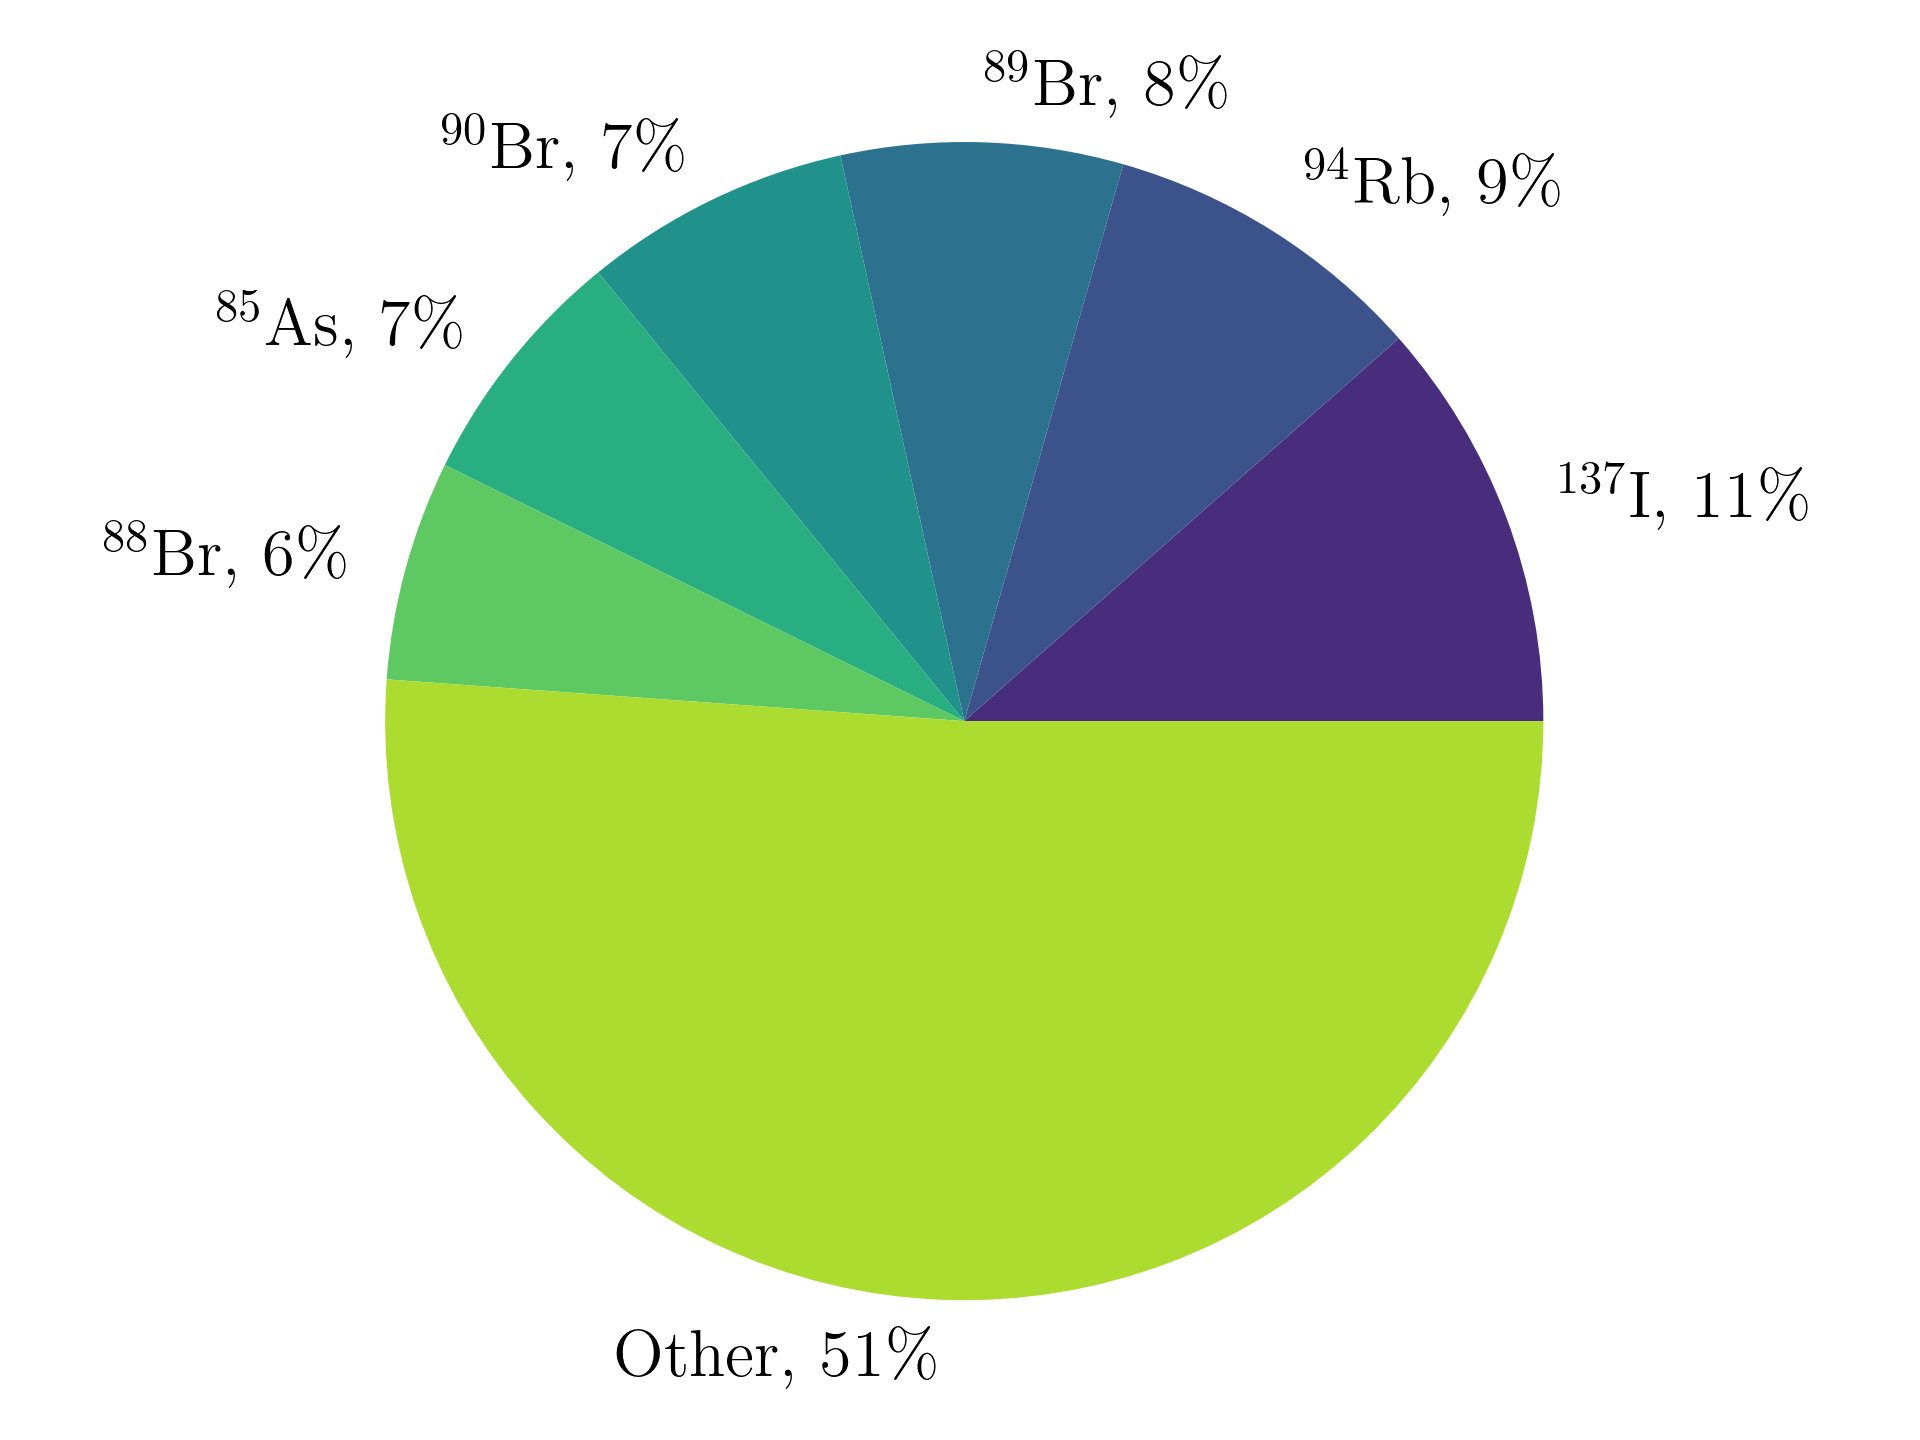
\includegraphics[width=0.5\linewidth]{images/b71/dnp_yield.png}
    \caption{The fraction of the delayed neutron yield from particular \glspl{DNP} from ENDF/B-VII.1 nuclear data. The six \glspl{DNP} with the largest delayed neutron yield contributions approximately 50\% of the total delayed neutrons per fission event. The remaining 212 \glspl{DNP} provide approximately 50\% of the total delayed neutron yield.}
    \label{fig:b71-dnp-yield}
\end{figure}


Table \ref{tab:b71-yld-hl} shows how the total delayed neutron yield $\nu_d$ and average half-life $\bar{\tau}$ compares between the value from the $I$ \glspl{DNP} and the six \gls{DNP} groups.
The differences between both are well within the uncertainty bounds, indicating the six groups are sufficiently capturing the general behavior of the delayed neutrons.
However, the average half-life differs by approximately two seconds from Section \ref{sec:iaea-jendl5}, while the total delayed neutron yield differs by approximately 300 $pcm$.


\begin{table}[]
    \centering
    \caption{ENDF/B-VII.1 nuclear data delayed neutron yield and average half-life values.}
    \begin{tabular}{lrl}
        \hline
        Parameter & Value & Units\\
        \hline
        $\nu_d(I)$ & $0.0191 \pm 0.0011$ &$ [-]$\\
        $\nu_d(K)$ & $0.0191 \pm 0.0009$ & $[-]$\\
        $\Delta \nu_d$ & $4.36 \pm 135.24$ & $[pcm]$\\
        \hline
        $\bar{\tau} (I)$ & $7.2 \pm 0.3$ & $[s]$\\
        $\bar{\tau} (K)$ & $7.2 \pm 0.3$ & $[s]$\\
        $\Delta \bar{\tau}$ & $0.01 \pm 0.4$ & $[s]$\\
        \hline
    \end{tabular}
    \label{tab:b71-yld-hl}
\end{table}

Table \ref{tab:b71-PCCi} shows the ten largest $PCC_i$ terms, which reveals which \glspl{DNP} have the greatest impact on the \gls{DNP} group parameters $\nu_{d,k}$ and $\tau_k$.
These results show that several \glspl{DNP} have a stronger correlation than $^{87}$Br, which is surprising considering its long half-life causes group one \gls{DNP} group parameters to be more sensitive to it.
However, differences in the emission probabilities, half-lives, and cumulative fission yields can cause \glspl{DNP} such as $^{137}$I to contribute more to \gls{DNP} group two.
For instance, Section \ref{sec:iaea-jendl5} shows that the \gls{PCC} for the group two half-life $\tau_2$ from changes in the $^{137}$I half-life is 0.726; but that same value calculated using the ENDF/B-VII.1 nuclear data is 0.922.

\begin{table}[]
    \centering
    \caption{ENDF/B-VII.1 nuclear data ten largest \glspl{PCC}.}
    \begin{tabular}{ll}
        \hline
       Nuclide & $PCC_{i}$ \\
       \hline
       $^{137}$I & 4.643721 \\
       $^{137}$Sb & 4.612421 \\
       $^{100}$Rb & 4.323455 \\
       $^{87}$Br & 3.604110 \\
       $^{85}$As & 3.025537 \\
       $^{88}$Br & 2.177990 \\
       $^{131}$Cd & 1.889176 \\
       $^{88}$As & 1.880888 \\
       $^{102}$Y & 1.311140 \\
       $^{89}$Br & 1.242374 \\
        \hline
    \end{tabular}
    \label{tab:b71-PCCi}
\end{table}

Table \ref{tab:b71-Ui} shows the ten largest $U_i$ terms, which corresponds to which \glspl{DNP} have the largest uncertainties relative to their impact on the \gls{DNP} group parameters $\nu_{d,k}$ and $\tau_k$.
There are several \glspl{DNP} that exist in both Table \ref{tab:b71-PCCi} and \ref{tab:b71-Ui}.
These \glspl{DNP} have a strong effect on the \gls{DNP} group parameters and have large relative uncertainties.
This means that, for ENDF/B-VII.1, these \glspl{DNP} will lead to greater uncertainty in the calculated \gls{DNP} group parameters and calculated delayed neutron emission rates. 

\begin{table}[]
    \centering
    \caption{ENDF/B-VII.1 nuclear data ten largest uncertainty-weighted \glspl{PCC}. Bold \glspl{DNP} are present in Table \ref{tab:b71-PCCi} as well, indicating they have a strong effect on \gls{DNP} group parameters.}
    \begin{tabular}{ll}
        \hline
       Nuclide & $U_{i}$ \\
       \hline
       \textbf{$^{100}$Rb} & \textbf{1.365283} \\
       \textbf{$^{137}$Sb} & \textbf{1.181643} \\
       $^{100}$Kr & 0.429832 \\
       $^{99}$Kr & 0.370420 \\
       \textbf{$^{102}$Y} & \textbf{0.320689} \\
       $^{87}$As & 0.307750 \\
       $^{124}$Ag & 0.275877 \\
       $^{124}$Pd & 0.254152 \\
       $^{84}$As & 0.249879 \\
       $^{147}$Xe & 0.241646 \\
        \hline
    \end{tabular}
    \label{tab:b71-Ui}
\end{table}

Figure \ref{fig:b71-bar-uiv} gives a more detailed view on which \gls{DNP} values specifically lead to the large $U_i$ values.
This offers slightly more insight than Table \ref{tab:b71-Ui}, which sums over the various \gls{DNP} values.
These results indicate that the half-lives are the primary sources of uncertainty that most affect the \gls{DNP} group parameters.
The top two \gls{DNP} in Table \ref{tab:b71-Ui} appear twice in this figure, as they have contributions from both the half-life nuclear data and their concentration.
The nuclear data for $^{100}$Rb and $^{137}$Sb are the most problematic in ENDF/B-VII.1 when calculating \gls{DNP} group parameters.


\begin{figure}
    \centering
    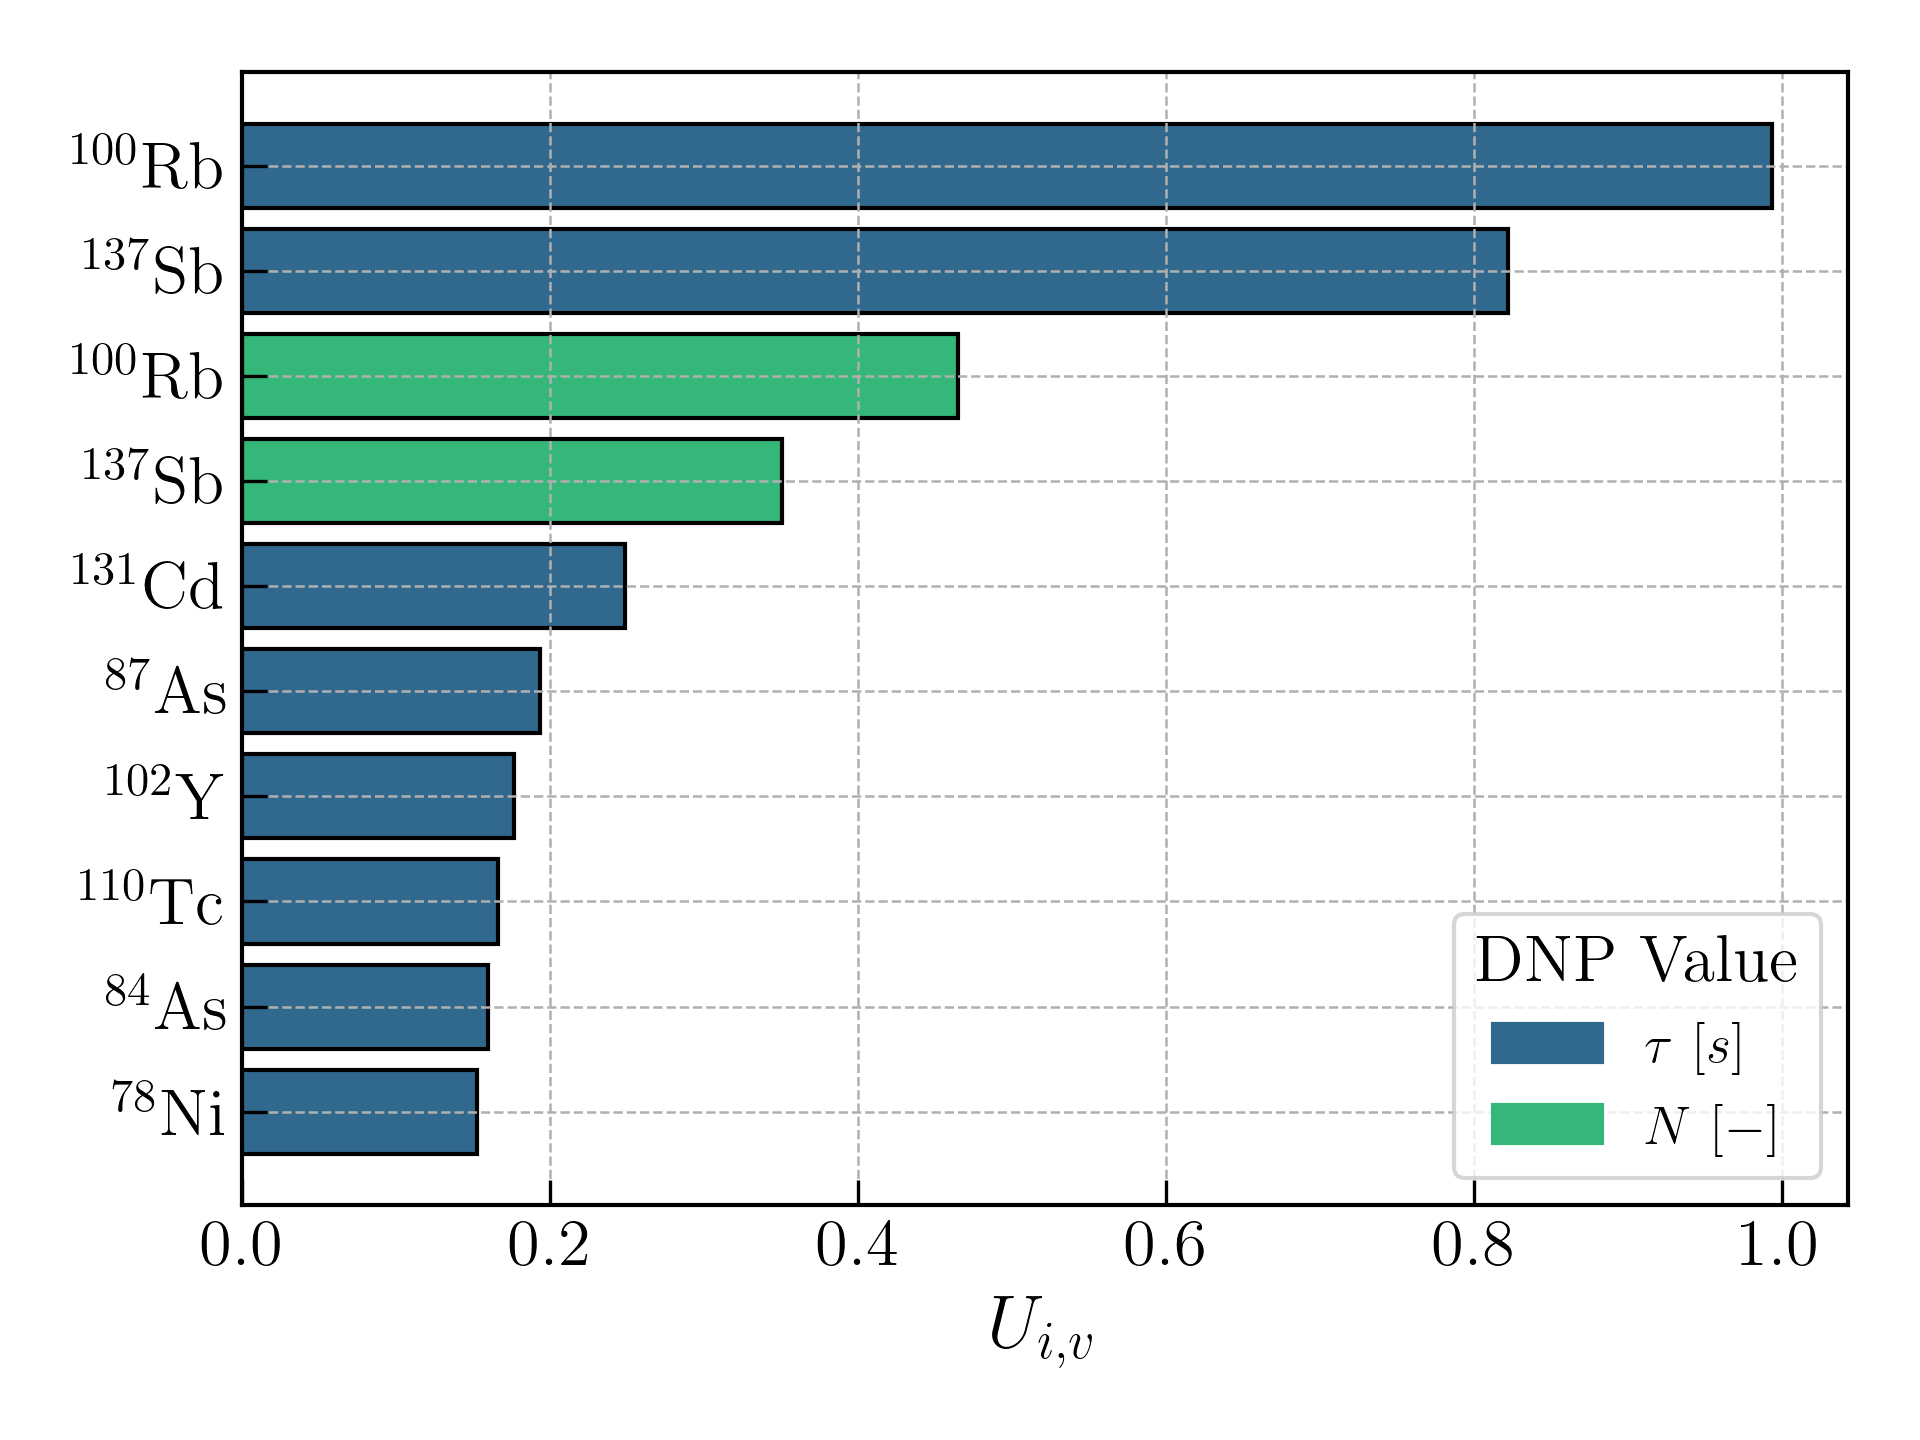
\includegraphics[width=0.5\linewidth]{images/b71/pcc-bar.png}
    \caption{The ten largest uncertainty-weighted \glspl{PCC} $U_{i,v}$ sorted by \gls{DNP} and associated \gls{DNP} value from JENDL-5 cumulative fission yields and IAEA beta-delayed neutron emission database half-lives and emission probabilities.}
    \label{fig:b71-bar-uiv}
\end{figure}


Figure \ref{fig:pcc-charts-b71} shows the $PCC_i$ and $U_i$ plotted on the chart of the nuclides.
These plots do not limit to only the top ten largest values, but instead show how all of the values compare among each other.
The values of $U_i$ are all smaller than those of $PCC_i$, because all of the relative uncertainties are less than 1.
There are two points of interest that have large $PCC_i$ and $U_i$ values, $^{100}$Rb and $^{137}$Sb, which can be seen on both plots.

\begin{figure}[!ht]
\centering
\subfloat[The $PCC_i$, or total \gls{PCC}, calculated for each \gls{DNP}.]{
  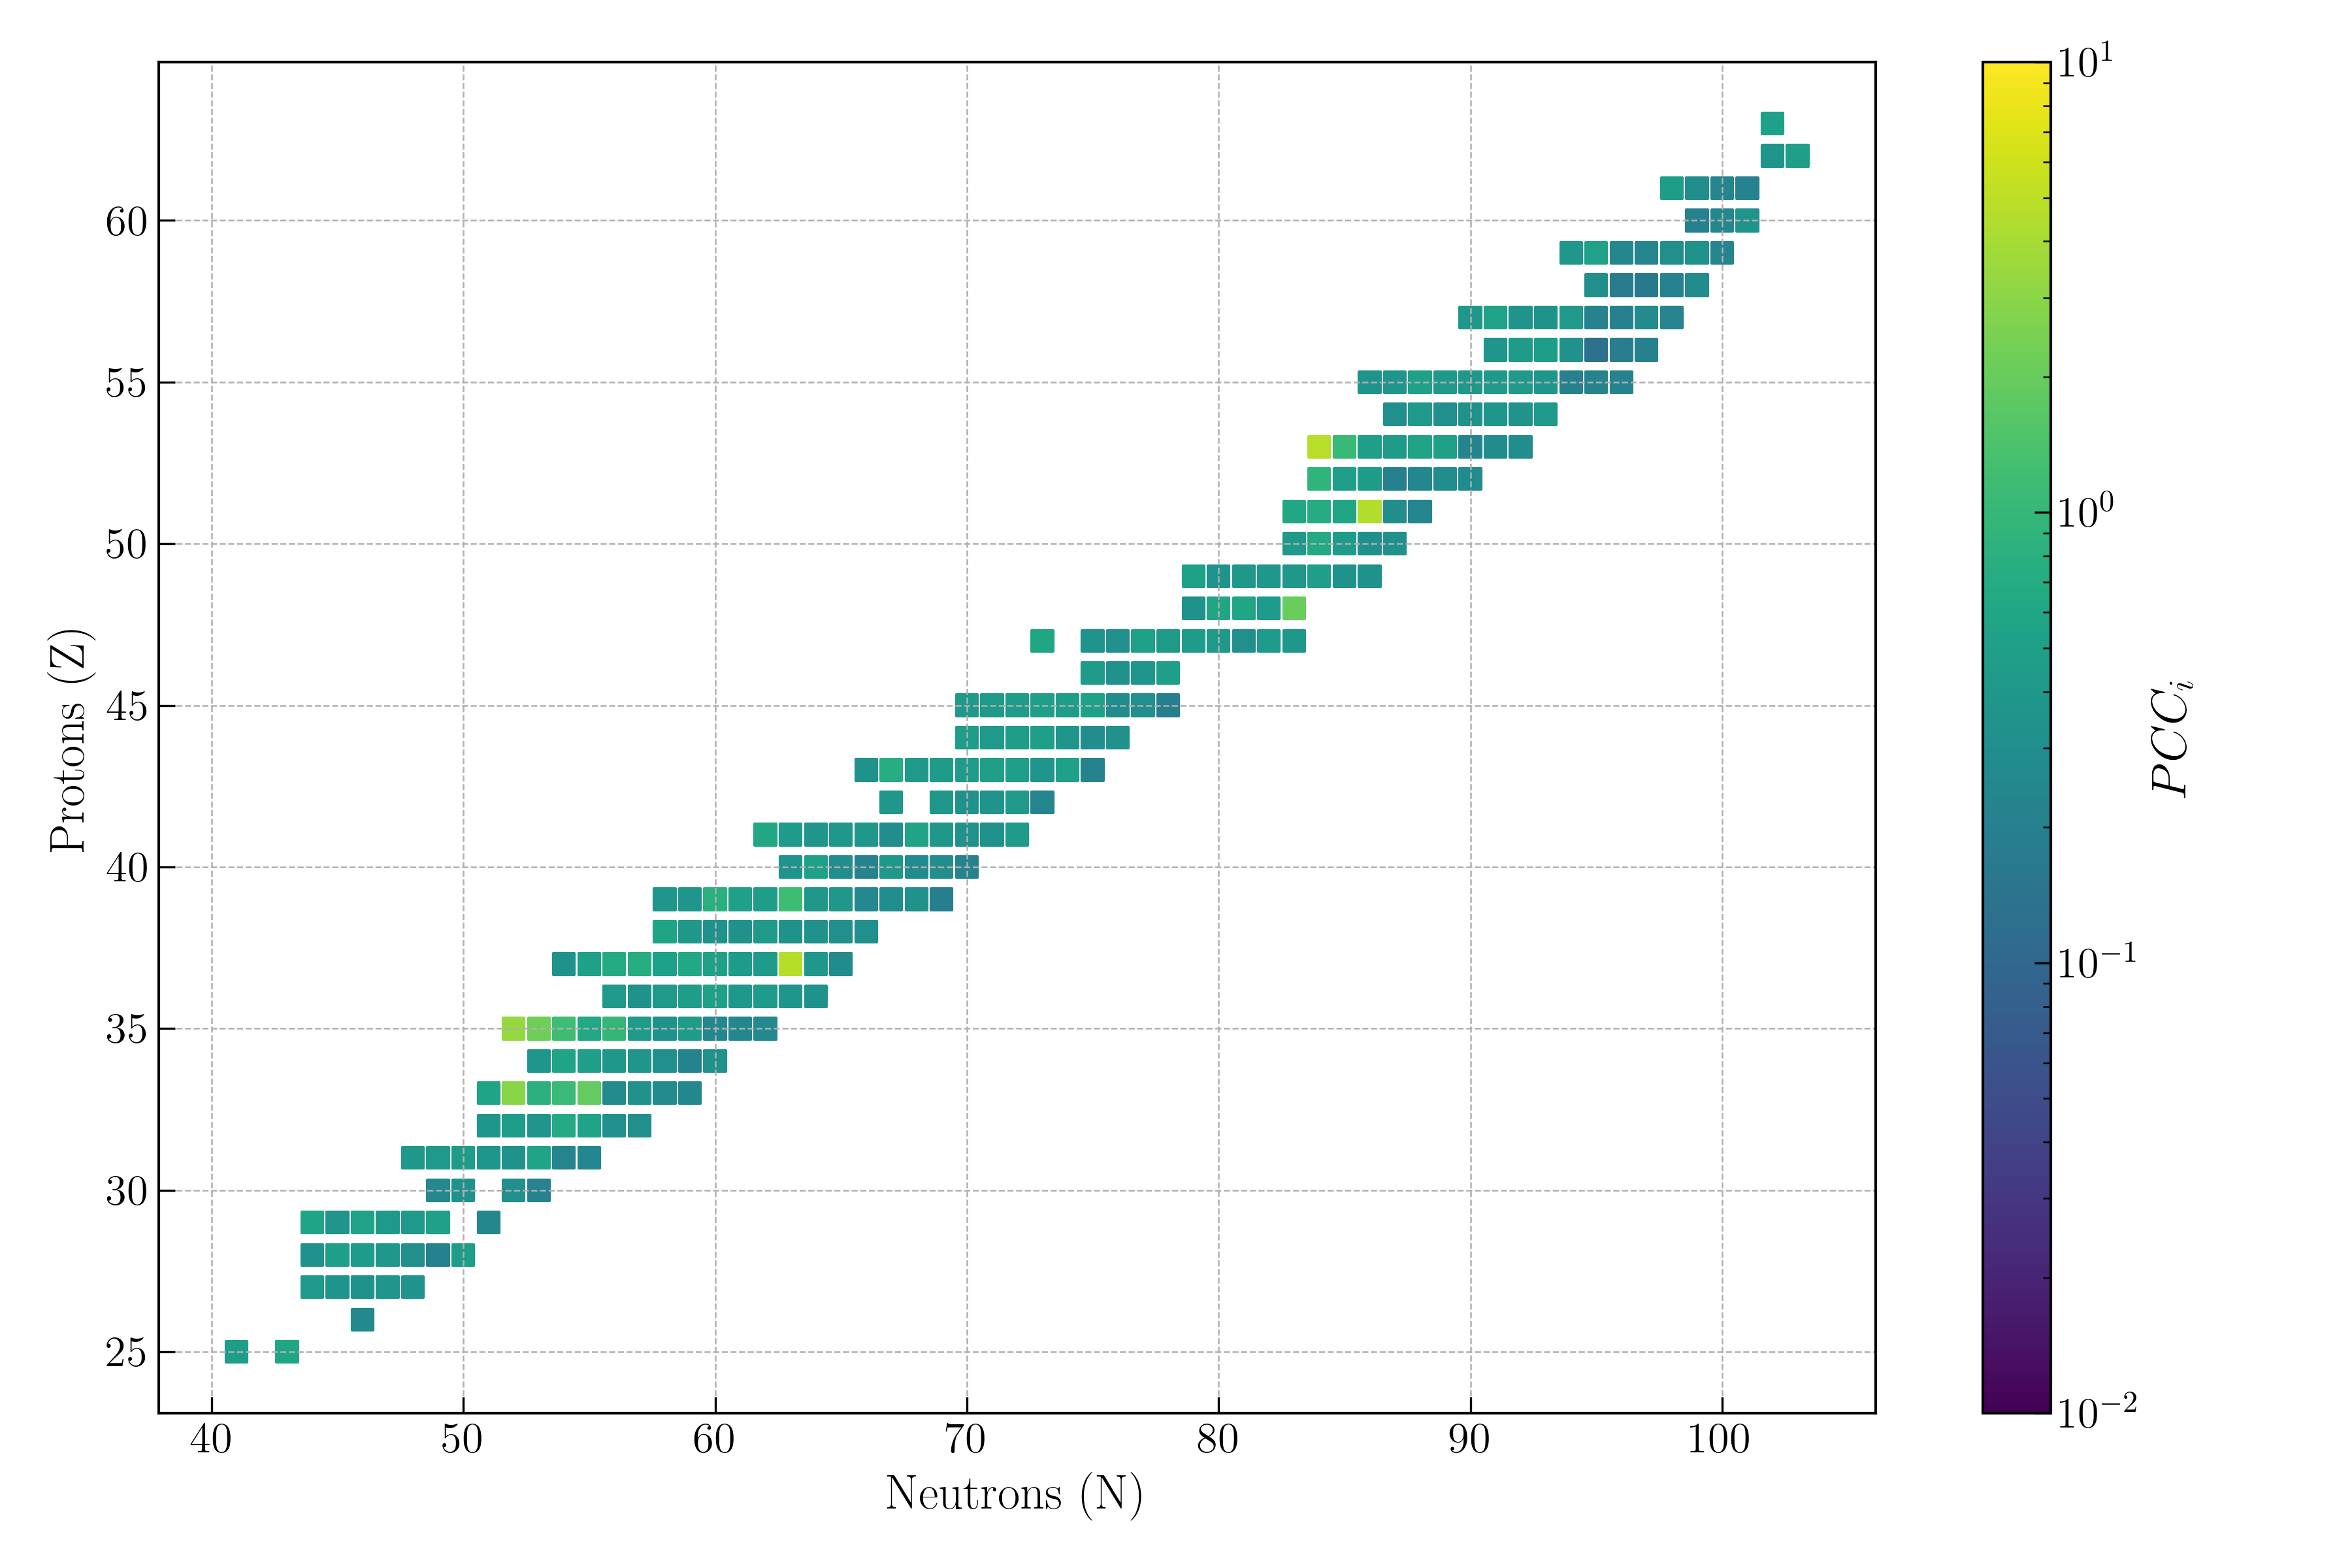
\includegraphics[width=0.45\linewidth]{images/b71/chart_PCC.png}
}
\hspace{0.05\linewidth}
\subfloat[The $U_i$, or total uncertainty-weighted \gls{PCC}, for each \gls{DNP}.]{
  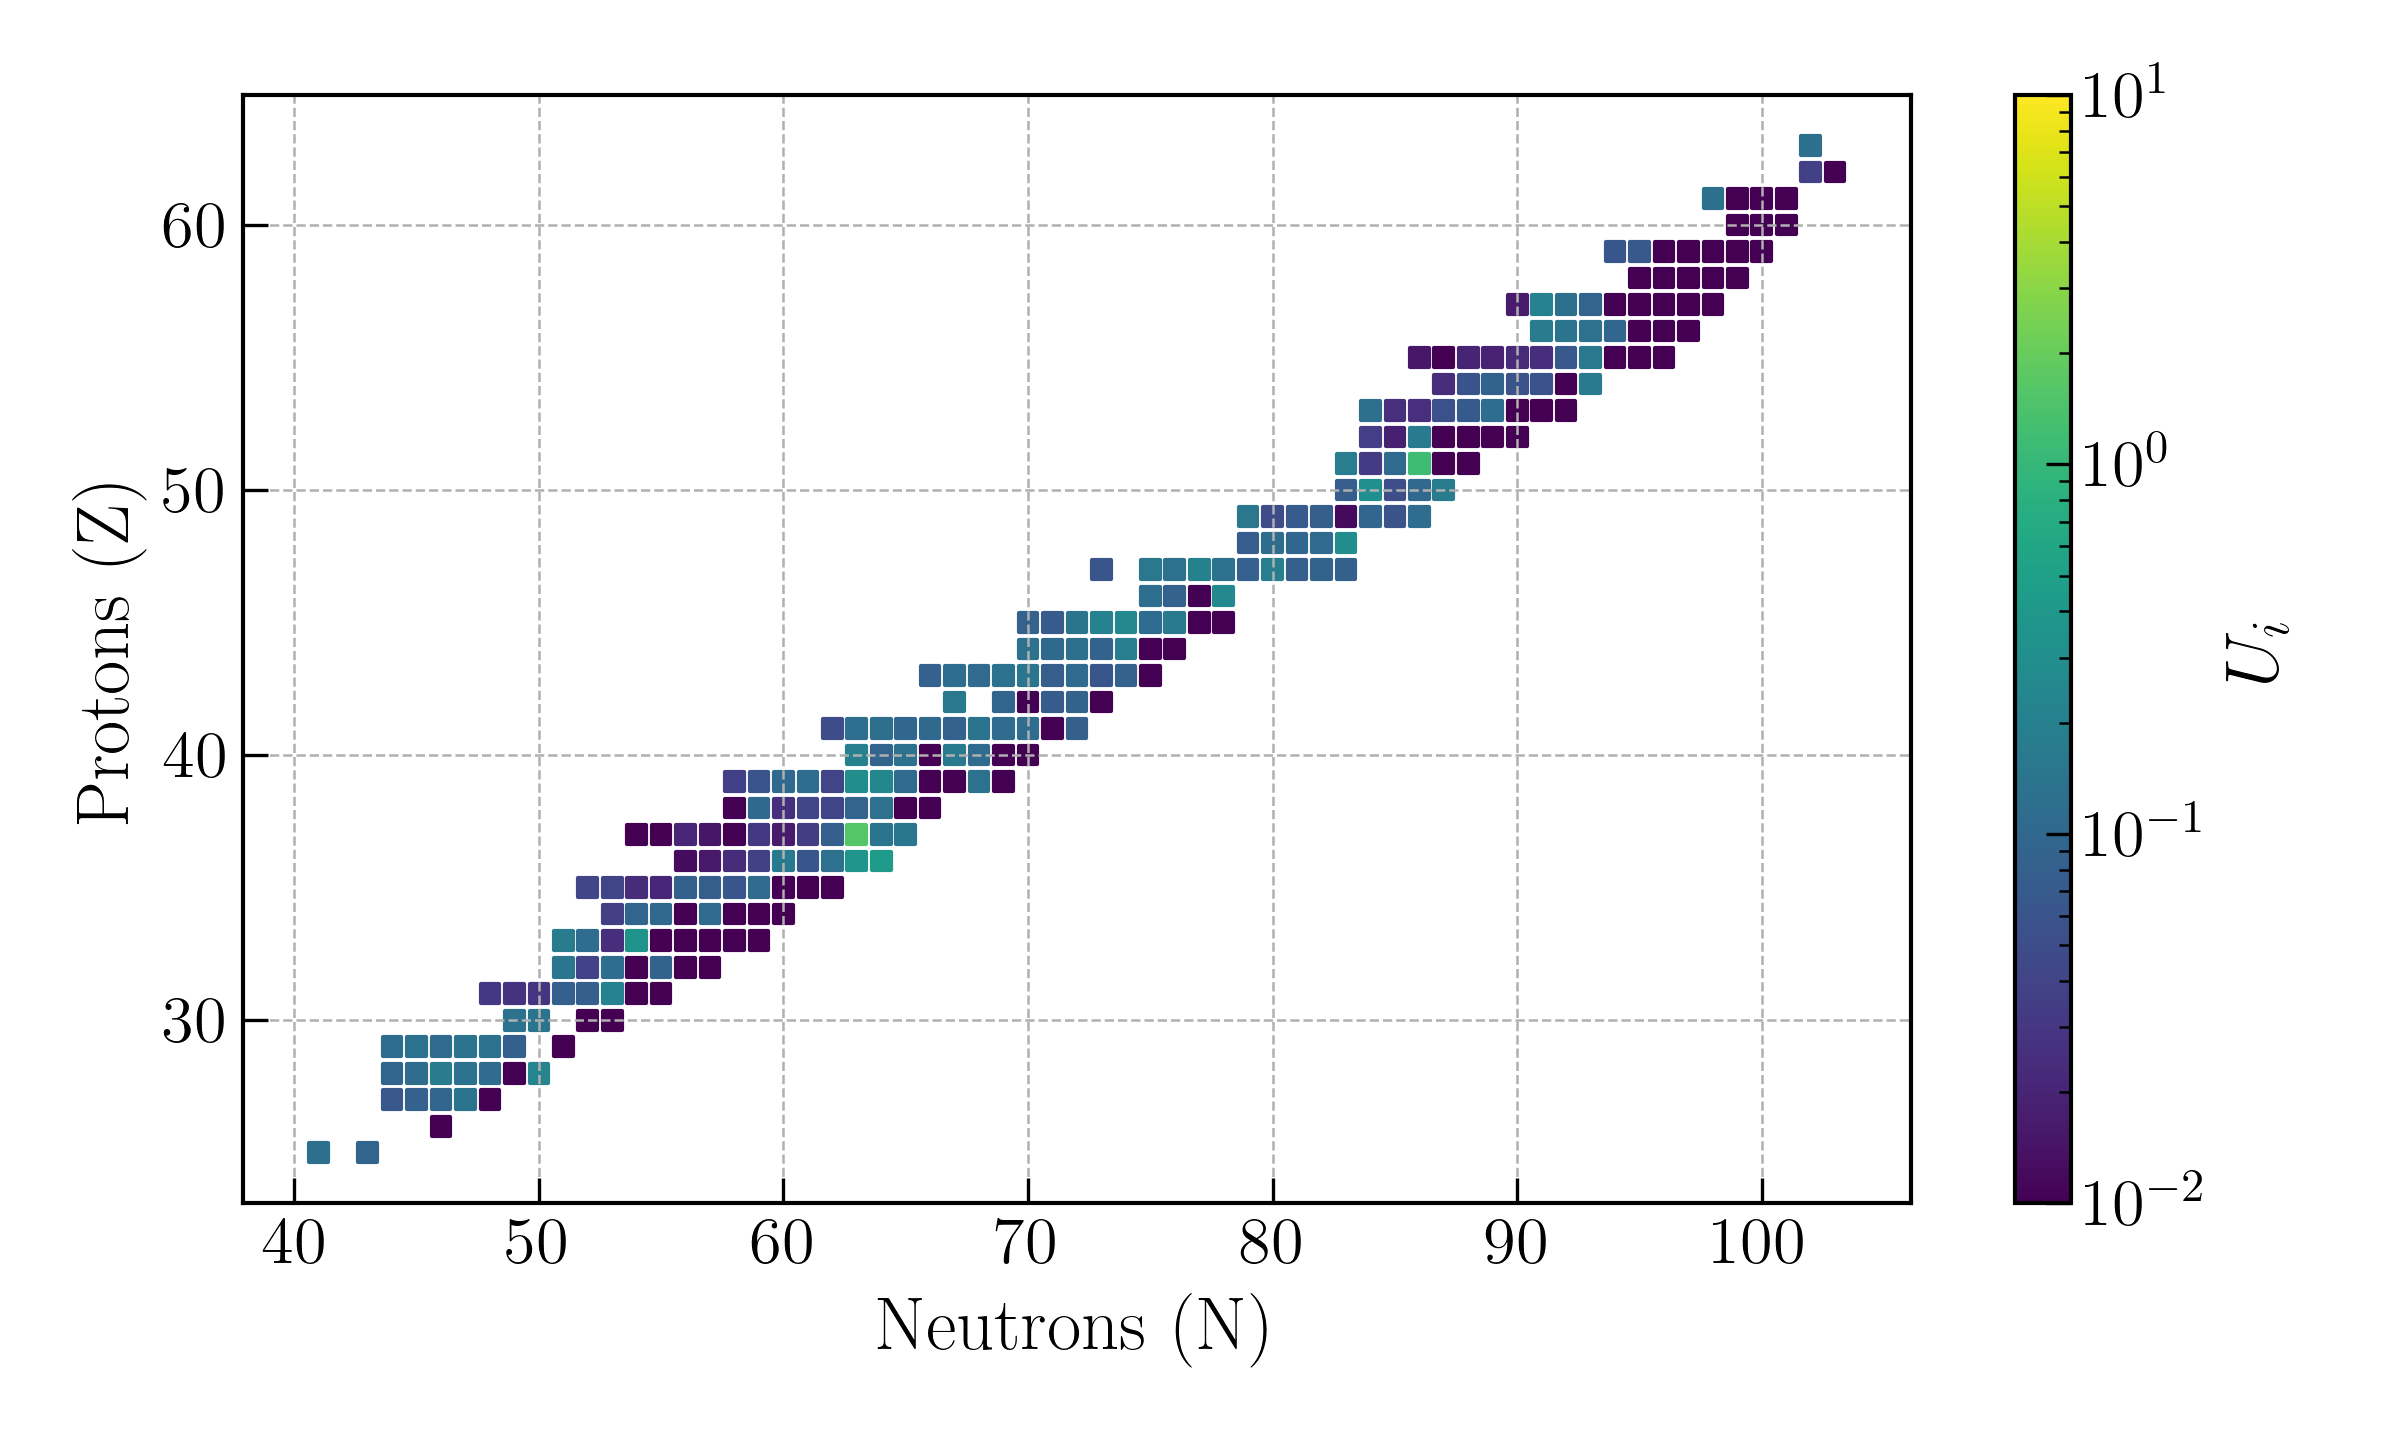
\includegraphics[width=0.45\linewidth]{images/b71/chart_PCC_uncertainty.png}
}
\caption{Chart of nuclide plots showing the \glspl{PCC} and uncertainty-weighted \glspl{PCC} using ENDF/B-VII.1 nuclear data.}
\label{fig:pcc-charts-b71}
\end{figure}



\FloatBarrier